\documentclass[T0_MEM]{subfiles}
\begin{document}

\section*{Figures}

% Figure 1 -----------------
\begin{figure}[!h]
  \centering
  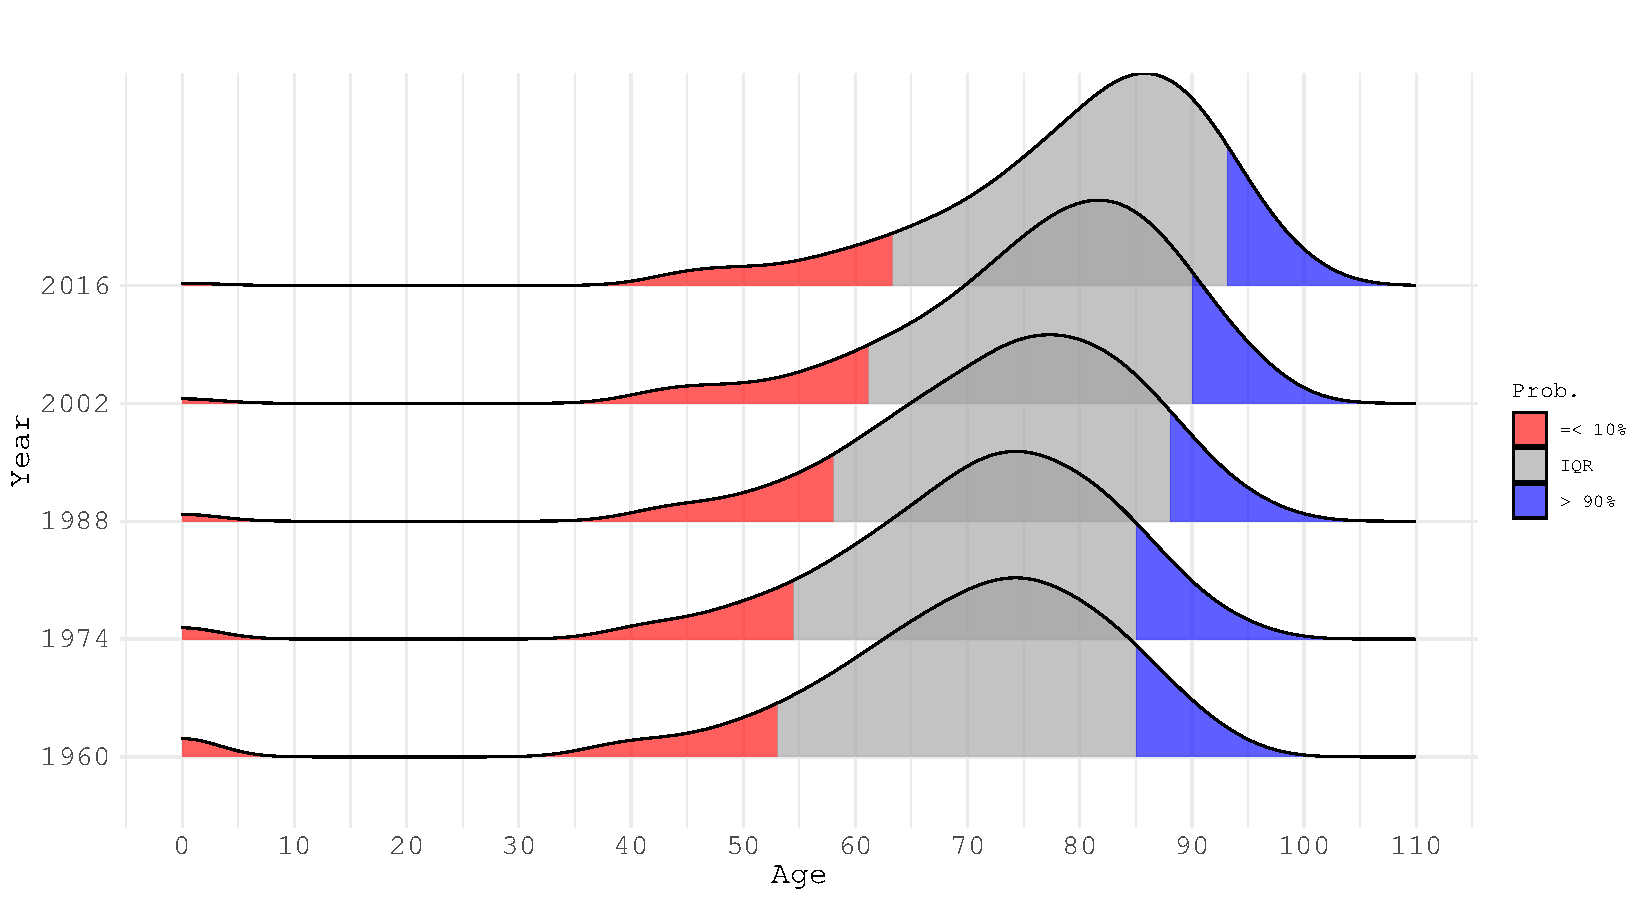
\includegraphics[width=1\linewidth]{figure/Figure-ObservedDx}
  \caption{\textit{Convergence of the age--at--death distribution
  (England \& Wales, Male population)}}
  \label{fig:ObservedDx}
\end{figure}

% Figure 2 -----------------
\begin{figure}[!h]
  \centering
  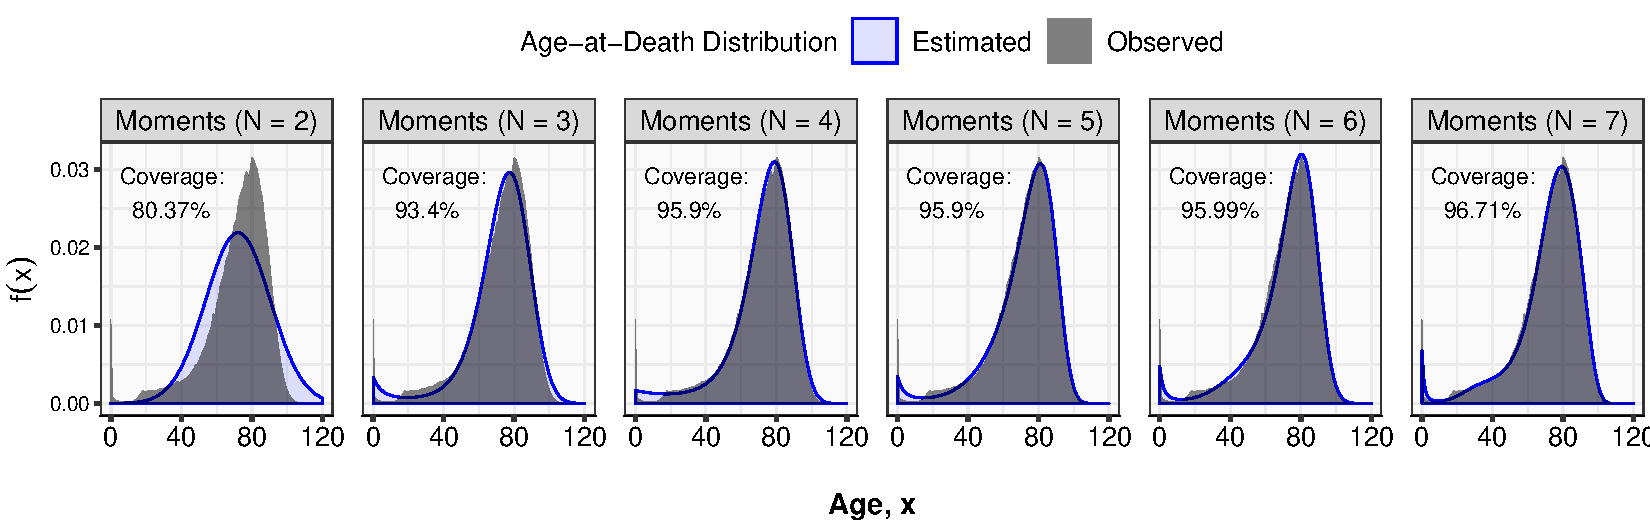
\includegraphics[width=1\linewidth]{figure/Figure-Convergence}
  \caption{\textit{Observed and estimated empirical density functions
  (USA, 1990, Male population)}}
  \label{fig:P_coverage}
\end{figure}

% Figure 3 -----------------
\begin{figure}[!h]
  \centering
  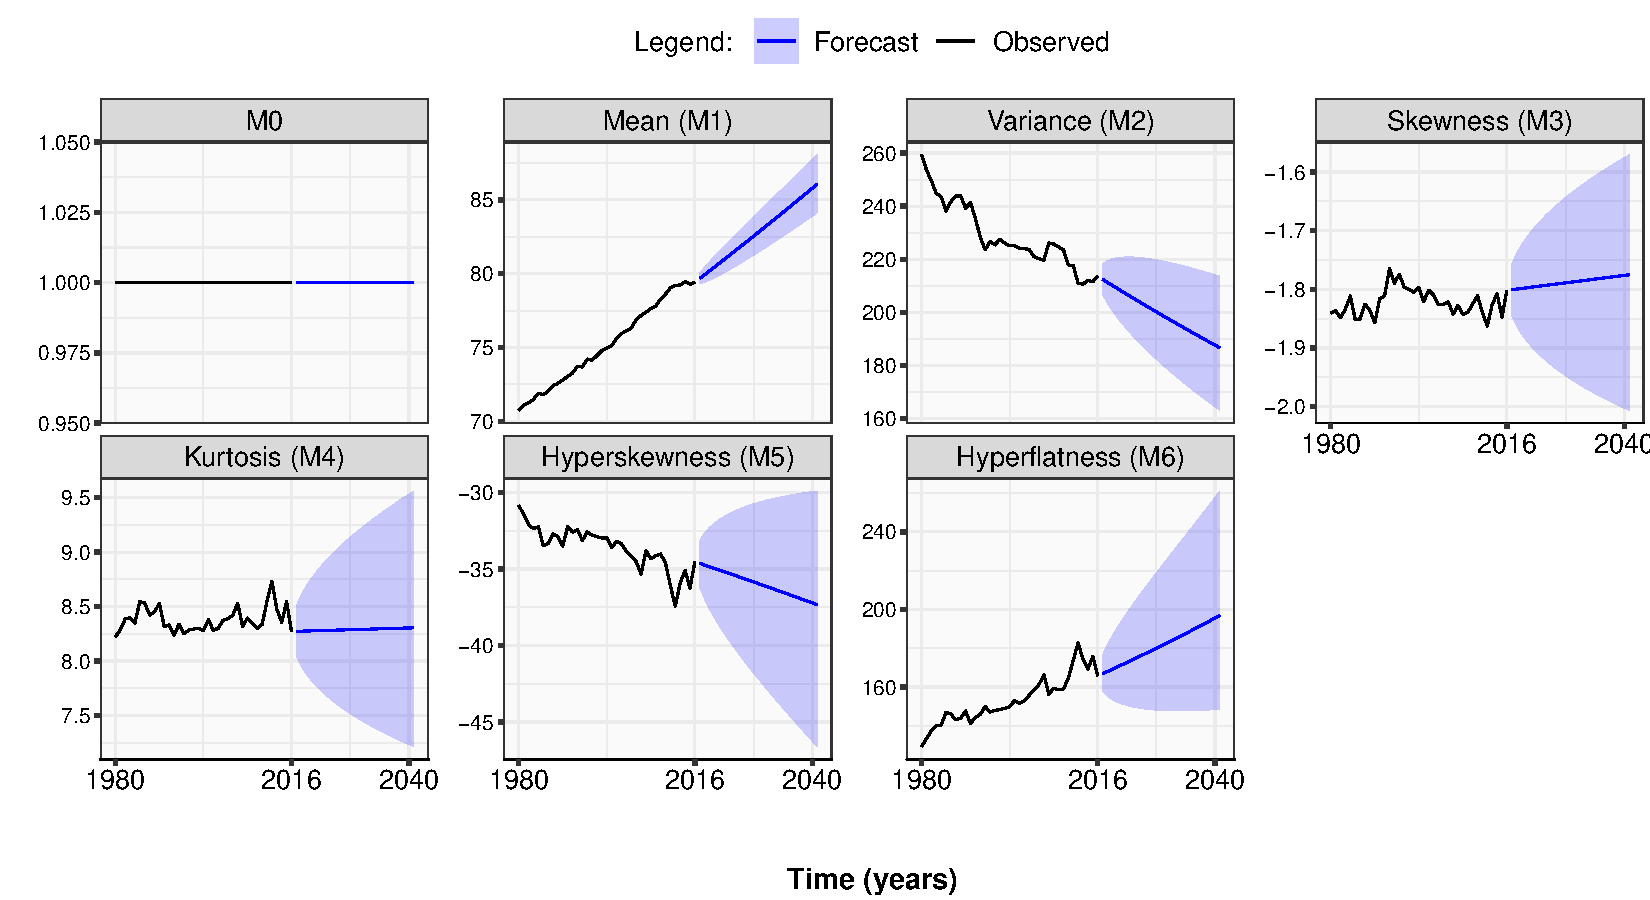
\includegraphics[width=1\linewidth]{figure/Figure-Moments}
  \caption{\textit{Forecast of statistical moments of the life table distribution of deaths together with 95\% prediction intervals, using a multivariate random--walk model (England \&Wales, Male population, 1980--2040)}}
  \label{fig:Moments}
\end{figure}

% Figure 4 -----------------
\begin{figure}[!h]
  \centering
  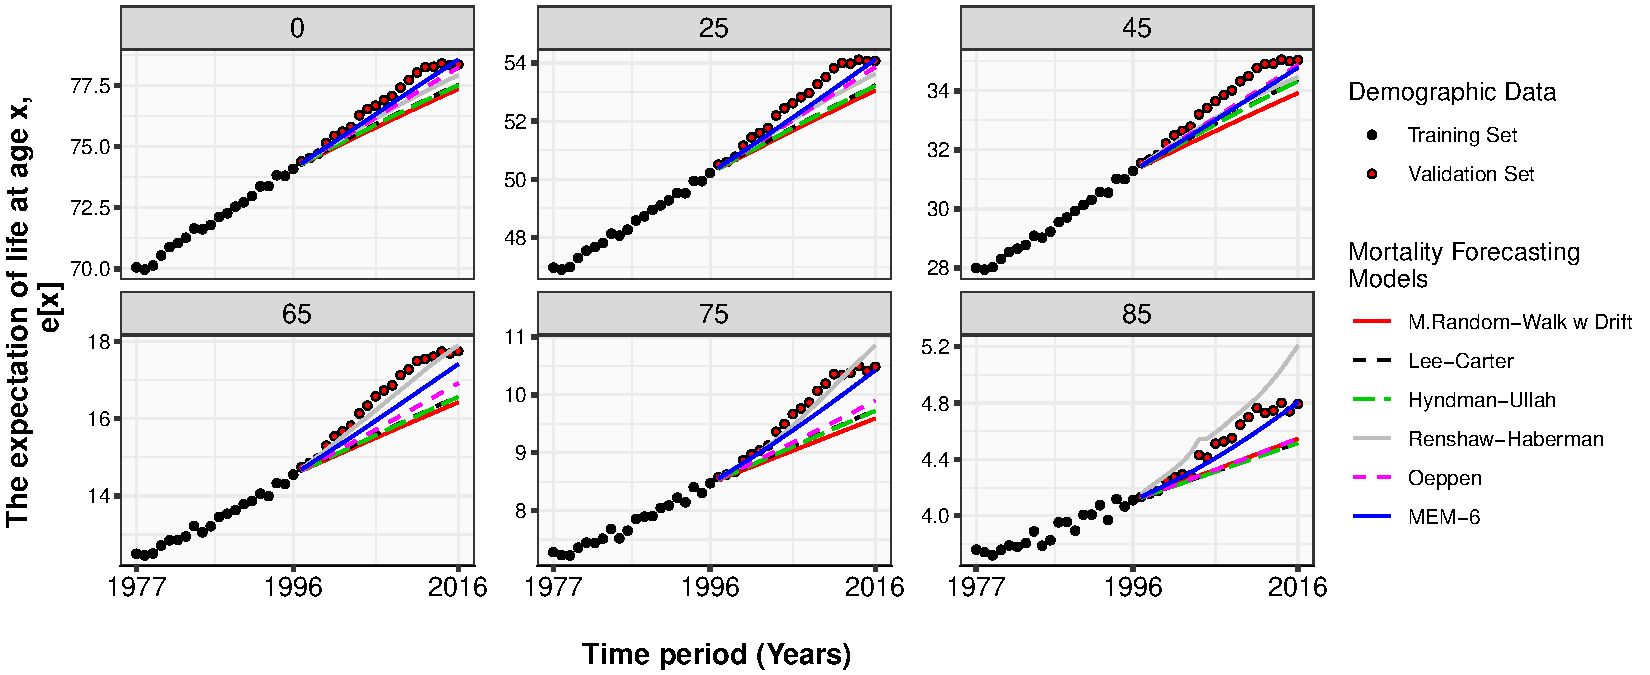
\includegraphics[width=1\linewidth]{figure/Figure_GBRTENW_ex}
  \caption{\textit{Out--of--sample forecast of the remaining life expectancy at various ages using the five mortality models (England \& Wales, Male population, Scenario 18: 1977--1996--2016)}}
  \label{fig:Forecast_ex}
\end{figure}

% Figure 5 -----------------
\begin{figure}[!h]
  \centering
  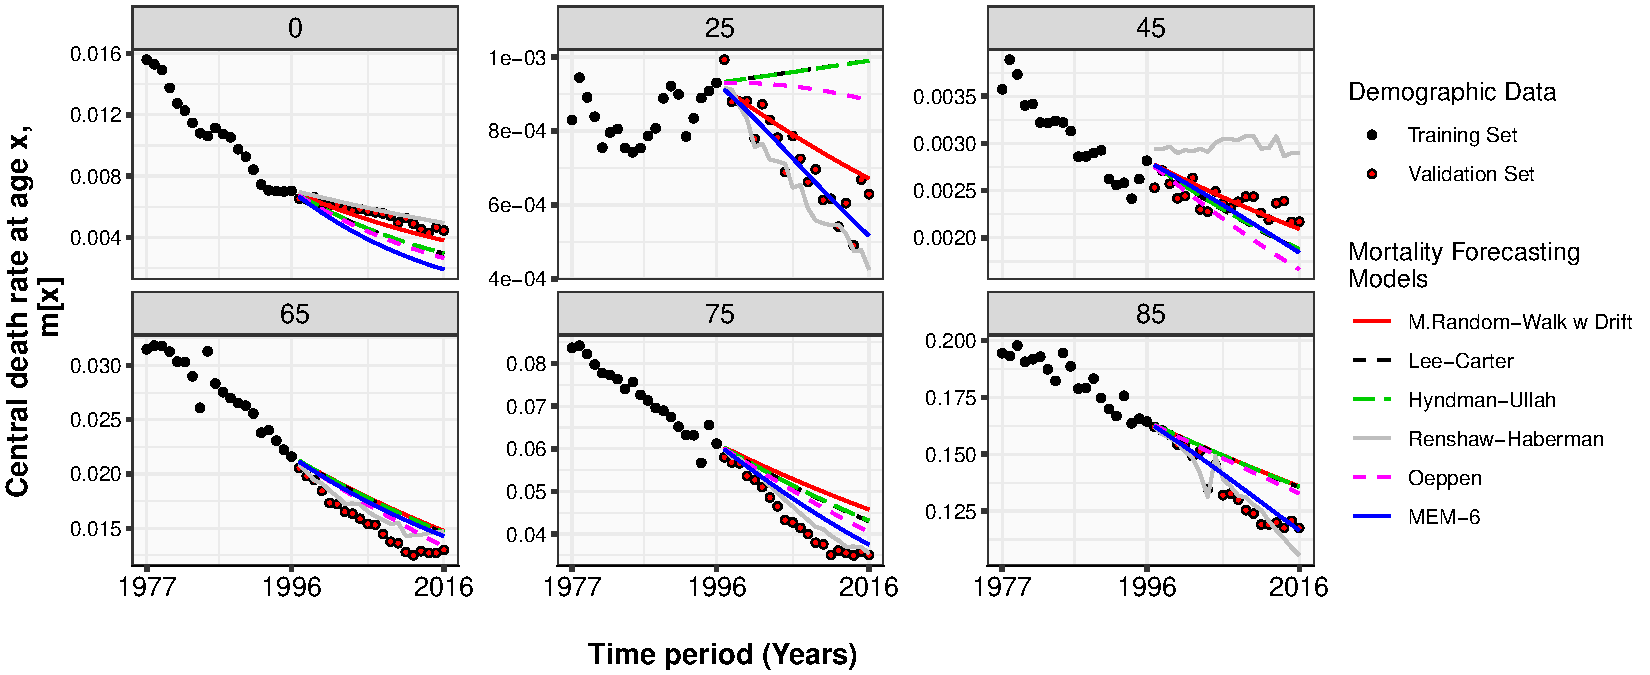
\includegraphics[width=1\linewidth]{figure/Figure_GBRTENW_mx}
  \caption{\textit{Out--of--sample forecast of the age-specific death rates using the five mortality models (England \& Wales, Male population, Scenario 18: 1977--1996--2016)}}
  \label{fig:Forecast_mx}
\end{figure}


\end{document}
